\documentclass[twocolumn,11pt]{IEEEtran}
\usepackage{epsfig}
\usepackage{amssymb}
\usepackage{amsmath}

%-----------------------

\begin{document}


\title{Insecurity of WEP}


\author{Arne Bjune and Vegar Engen \\ \texttt{\{arnedab,vegaen\}@cs.ucsb.edu}}

\markboth{Insecurity of WEP}{Bjune and Engen}

\maketitle

\begin{abstract}
802.11 has included Wired Equivalent Privacy (WEP) protocol, used to protect the link-layer communication from attacks. Several years ago critical security flaws were discovered, which compromises message transmission in WEP secured networks. In this paper we will discuss how WEP works, why it is broken, and how it the security issues could have been avoided.
\end{abstract}

\section {Introduction}
\label{sec:introduction}

%% Something about increase of devices 

In the last decade the increase of mobile devices has been enormous, and to be connected to the Internet is required in a lot of daily activities.  with a wide specter of devices. To easily be able to connect to Internet with this wide spectrum of devices, wireless networks have been popular. But this new won freedom raises newer problems, is it secure to connect to a wireless network? Since we in wireless networks are transmitting data through radio waves, in contrast to a wired network were we transmitting data through a cable, the communication is a easier to intercept. Hence wireless network communication is in need for a way to protect the communication. \\


With the objective to enforce the security issues Wired Equivalent Privacy (WEP) protocol was introduced and described in 802.11 standard\cite{IEEE:Fast} for wireless networks. The most important goal assigned to WEP was to ensure the users confidentiality from casual eavesdropping.In addition two other main goals were added. First WEP was supposed to take care of access control, so only entrusted users were able to connect to the wireless infrastructure. The last goal was that WEP should ensure that data transmitted was not tampered with.   \\


Unfortunately, WEP was not able to live up to its expectation, since it came too short to accomplish any of its main goals. Even though it was based on a well known and tested RC4 stream cipher, a poor design choice was enough to make WEP contain major security flaws. Those flaws make it possible to tampering, and eavesdrop on the wireless transmission. We will discuss attacks more in detail in section ??????. \\



This paper is organized as following: We will start with the introduction in 
section \ref{sec:introduction}, then a brief explanation of what WEP is in 
section \ref{sec:whatiswep}. 


\section {What is WEP?}
\label{sec:whatiswep}

Wired Equivalent Privacy (WEP) is a protocol described in the documentation of 802.11 for wireless networks. WEP is used to protect link-layer transmissions from attacks. WEP uses a shared secret key \emph{k} to protect the data sent between the to parts. The protocol does also make a checksum \emph{c(M)} of the message. The plain text that is going to be encrypted is \emph{P = M, c(M)}. 



\section {The Goals of WEP}
\label{sec:goals}

The WEP protocol was not design to give ultimate security, but rather equal to wired networks. To be able to enforce the security a few security goals had to be defined\cite{IEEE:Fast}:\\

\begin{description}
\item[Confidentiality:] The most important feature of WEP is that it is have to prevent eavesdropping.
\item[Access Control:] Another important goal of WEP is that only authorized devices are able to connect to the wireless infrastructure. The 802.11 protocol does also include a feature which can drop all packets that are not WEP encrypted.
\item[Data integrity:] It is also important that the data transmission isn't tampered with. To be able to enforce this the checksum is added.\\
\end{description}


For all the goals the claimed security is ``based on the difficulty of obtaining the secret key through brute-force'' \cite{IEEE:Fast}



\section {WEP Encryption}
\label{sec:WEP_Encryption}

WEP uses a stream cipher called RC4 to protect the data transmitted over a wireless link. RC4 was invented in 1987 by Ron Rivest and is widely used to protect network traffic. The seed for the RC4 stream cipher is 64 or 128 bits consisting of a 24 bit initialization vector and a 40/104 bit key. The key is normally represented as a 10/26 character hex values. A alternative way to represent the key is 5/13 ASCII characters but that reduces the key space with a factor of approximately 2.5 (95 vs 256 possible values for 8 bits).

A stream cipher produces a psudo random stream of bits which is then xored with the plaintext and transmitted to the receiver that runs the same algorithm and xores again to get the plaintext. A known problem with stream cipher is using the same key again. To avoid key stream reuse WEP was designed with a 24 bit initialization vector (IV) that is concatenated with the secret key to make the seed for the RC4 cipher. However the 802.11 standard says nothing about how IV should be chosen. Just using the same IV for every packet is a valid implementation according to the specification. A implementation choosing IV at random will have a collision every 5000 packets\cite{Borisov:New}. A busy access point with optimal IV management would still go through the entire IV keyspace in a single day.

The problem with two packets using the same IV is that they will use the same keystream. So its vulnerable to a Known Plaintext Attack.


\begin{align*}
C = P \oplus RC4(IV,key) \\ \\
C1 \oplus C2 = \\
(P1 \oplus RC4(IV,key) ) \oplus ( P2 \oplus RC4(IV,key)) \\
= P1 \oplus P2
\end{align*}

So if you know P1 it is trivial to find P2. 

\begin{figure}
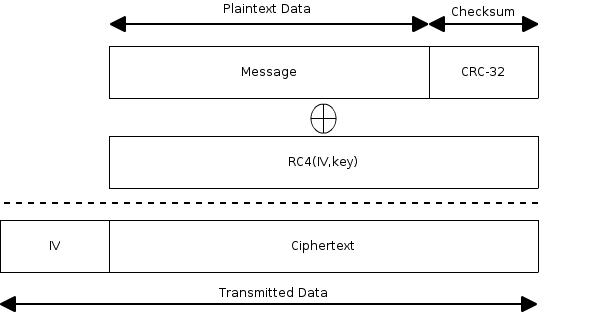
\includegraphics[width=90mm]{WEP_Encryption.png}
\caption{WEP Encryption}
\end{figure}

In WEP the IV is sent in plaintext together with the package so there is easy for an attacker to find colliding packets. Even without knowing the plaintext of a message it is possible to find plaintext candidates because of the predictability of packet headers. Also the first packets a new host sends to the network are predictable. For example DHCP leases and login sessions. As an attacker discovers more and more keystreams storing keystreams of all possible IV is an option. Assuming 1500byte packages the $2^24$ possble combinations will only take 24GB of space to store.

\section {Conclusion}
\label{sec:conclusion}

Here we need space for the conclusion



\section {Future}
\label{sec:future}

WEP is now depreciated and has been replaced with WPA (802.11i draft) and WPA2 (802.11i-2004). WPA/WPA2 provides significantly improvements in security as well new ways of authenticating with the access point. The ability to have a central point  of authentication and support for RADIUS is crucial in a corporate environment.




\bibliographystyle{IEEEbib}
\bibliography{my}


\end{document}
